% Created 2020-11-27 ven. 10:07
% Intended LaTeX compiler: pdflatex
\documentclass[a4paper]{article}
\usepackage[utf8]{inputenc}
\usepackage[T1]{fontenc}
\usepackage{graphicx}
\usepackage{grffile}
\usepackage{longtable}
\usepackage{wrapfig}
\usepackage{rotating}
\usepackage[normalem]{ulem}
\usepackage{amsmath}
\usepackage{textcomp}
\usepackage{amssymb}
\usepackage{capt-of}
\usepackage{natbib}
%\usepackage{subfigure}
\usepackage{subcaption}
\usepackage[linktocpage,pdfstartview=FitH,colorlinks,
linkcolor=blue,anchorcolor=blue,
citecolor=blue,filecolor=blue,menucolor=blue,urlcolor=blue]{hyperref}
\usepackage{geometry}
\geometry{a4paper,total={170mm,257mm},left=10mm,	top=20mm,	rmargin = 20mm,	bottom = 20mm}
\usepackage{babel}
\newtheorem{theorem}{Theorem}
\newtheorem{corollary}{Corollary}
\newtheorem{lemma}[theorem]{Lemma}
\newtheorem{Proposition}{Proposition}
\newtheorem{Remark}{Remark}
\newtheorem{Assumption}{Assumption}
\newtheorem{Definition}{Definition}
\usepackage{graphicx}

\def\1{{\bf 1}_N}
\def\0{{\bf 0}}
\def\N{{\mathbb N}}
\def\R{{\mathbb R}}
\def\E{\mathcal{E}}
\def\G{\mathcal{G}}
\def\T{\mathcal{T}}
\def\I{\mathcal{I}}
\def\L{\mathcal{L}}
\def\P{\mathcal{P}}
\newcommand{\unn }{\{1,\ldots, n\}}
\newcommand{\unN}{\{1,\ldots, N\}}
%\author{Bikash Adhikari}
%\date{\today}
\title{Report: Synthesis of optimal filter for MHOQ} 
%\hypersetup{
% pdfauthor={Bikash Adhikari},
% pdftitle={Linear Quadratic Regulator (LQR)},
% pdfkeywords={},
% pdfsubject={},
% pdfcreator={Emacs 26.3 (Org mode 9.3.6)}, 
% pdflang={English}}


\begin{document}
\newpage
\maketitle
\tableofcontents

\section{Quantisation}
Let $w \in \mathbb{R}$ be the input, $\mathbf{Q}$ be the quantiser and $y \in \mathbb{U}$ the quantiser output. The quantiser output 
Let us define the quantisation error as 
\begin{equation}
	q = \mathbf{Q}(w) - w= y -w.
	\label{eq:error}
\end{equation}
The quantisation requires the signal to be mapped to a finite signal where each value of the output $y$ is restriced to belong to a finite set $\mathbb{U}$. The elements of the set $\mathbb{U}$ represent the quantiser levels and depends on the word-size of the quantiser. 

\section{Noise shaping quantiser}
Noise-shaping quantisers can reduce the effective quantisation error by moving quantisation noise to higher 
frequencies through oversampling and feedback.  The reconstruction filter is then used to attenuate the 
frequency-shaped quantisation noise. It operates by estimating the uniform quantisation error and employing a 
feedback filter to shape the noise power at the output of the DAC. A block diagram for a noise-shaping quantiser 
is shown in Fig. \ref{fig:dsm1}. The feedback filter $F(z)$ is designed such that the transfer 
function $y = (1 - F(z)) \epsilon$ is a high-pass filter.

\begin{figure}[!h]
	\centering
	\begin{minipage}{0.45\linewidth}
		\centering
		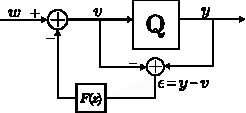
\includegraphics[scale = 1.5]{figures/noise_shaping2.pdf}
		\caption{Noise shaping quantiser}
		\label{fig:dsm}
	\end{minipage}
	\hfil  
	\begin{minipage}{0.45\linewidth}
		\centering
		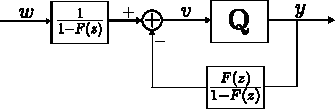
\includegraphics[scale = 1.5]{figures/noise_shaping_redrawn.pdf}
		\caption{Noise shaping quantiser}
		\label{fig:dsm1}
	\end{minipage}
\end{figure}



In linear analysis, the output is given by 
\begin{equation}
	Y(z) = \textbf{STF}. W(z) + \textbf{NTF} .E(Z)
\end{equation}
where the signal transfer function $\textbf{STF} = 1$, noise transfer function $\textbf{NTF} =  (1-F)$ 
and $F = z^{-1}$ for the first-order delta sigma modulator. 

\section{Moving horizon optimal quantiser (MHOQ)}
The design criteria for the MHOQ is the minimization of the perceived errors defined as follows:
\begin{equation}
	e(t) = H(z)(u(t)-y(t))
	\label{eq:error1}
\end{equation}
where  $H(z)$  is  a stable time-invariant linear low-pass filter with the following state-space
\begin{equation}
	\label{eq:filter_statespace}
	H(z) = 1 + C(z I - A)^{-1} B
\end{equation}
The error $e$  then can be written as the output of the following state-space representation of $H$
\begin{equation}
	\begin{aligned}
		x(t+1) &= A x(t) + B (u(t)-y(t))		\\
		e(t) &= Cx(t) + u(t)-y(t)
	\end{aligned}
	\label{eq:statespace1}
\end{equation}
where $x \in \mathbb{R}^{n}$ is the state vector.  The error $e$ corresponds to the difference between the filtered quantised signal and the filtered input signal. 

For moving horison implementation, the optimisation problem is defined as the problem of finding $y \in \mathbb{U}$ that minimises  the cost function  while satisfying the state equations as follows:
\begin{align}
		& y^{\ast}(t) = \arg  \min_{y(t) }	V_{N}  = \sum_{t=k}^{k+N-1} e^{2}(t) \\
		\intertext{subject to}
		&x(t+1) = A x(t) + B (y(t)-w(t))		\\
		&e(t) = Cx(t) + y(t)-w(t)		\\
		&y(t) \in \mathbb{U}.
	\end{align}

\section{Frequency response: LPF and NTF}
\subsection{Perception filter}
The  frequency response and the STF and NTF of the perception filter used in  
\cite{goodwin2003moving} are shown in the
figure below, 
\begin{figure}[!h]
	\centering
\begin{minipage}{0.45\linewidth}
	\centering
	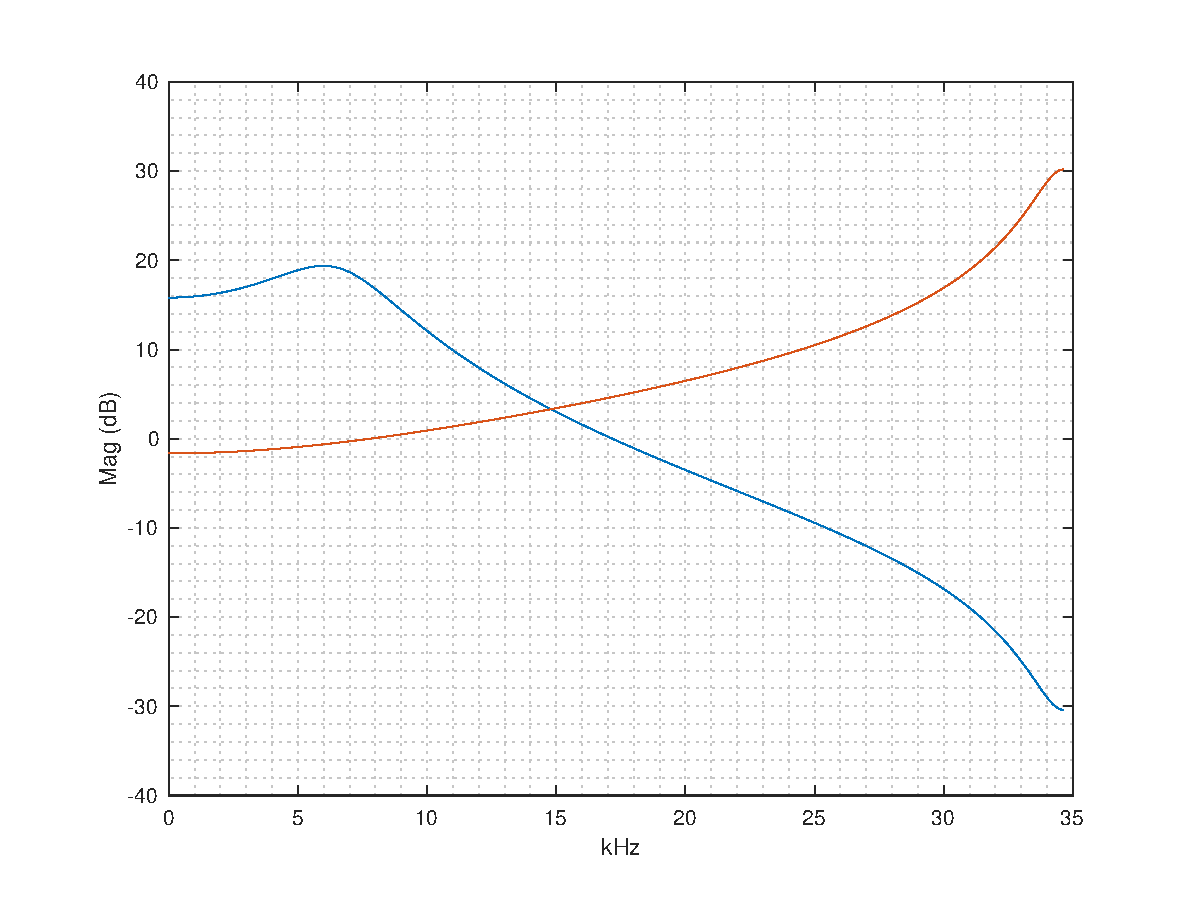
\includegraphics[scale = 0.45]{plots/percp.eps}
        \caption{Perception filter Frequency response}
	\end{minipage}
	\hfil
	\begin{minipage}{0.45\linewidth}
	\centering
	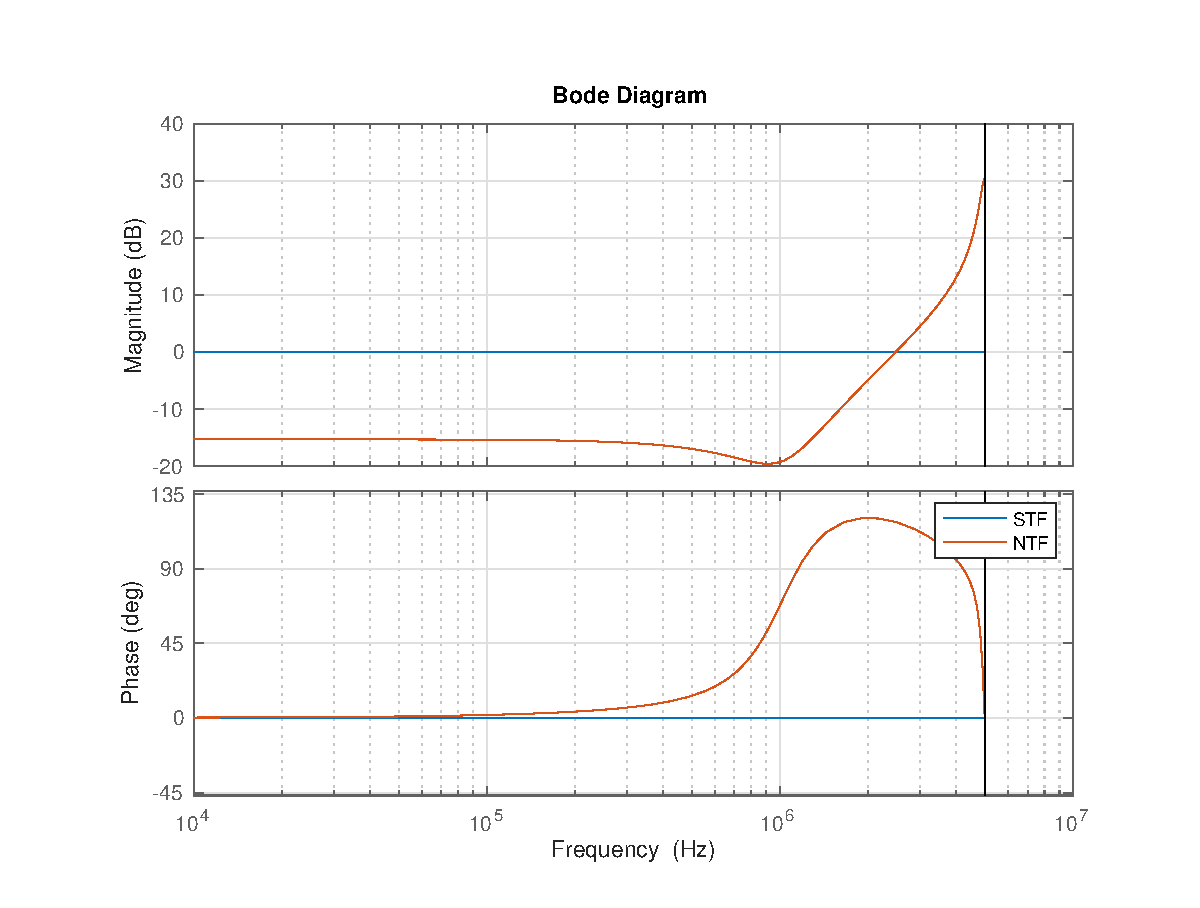
\includegraphics[scale = 0.45]{plots/stf_ntf_perception_linear.eps}
		\caption{STF and NTF using perception filter}
\end{minipage}
\end{figure}


% \subsection{Butterworth Filter}

% \begin{figure}[!h]
% 	\centering
% 	\begin{minipage}{0.45\linewidth}
% 		\centering
% 		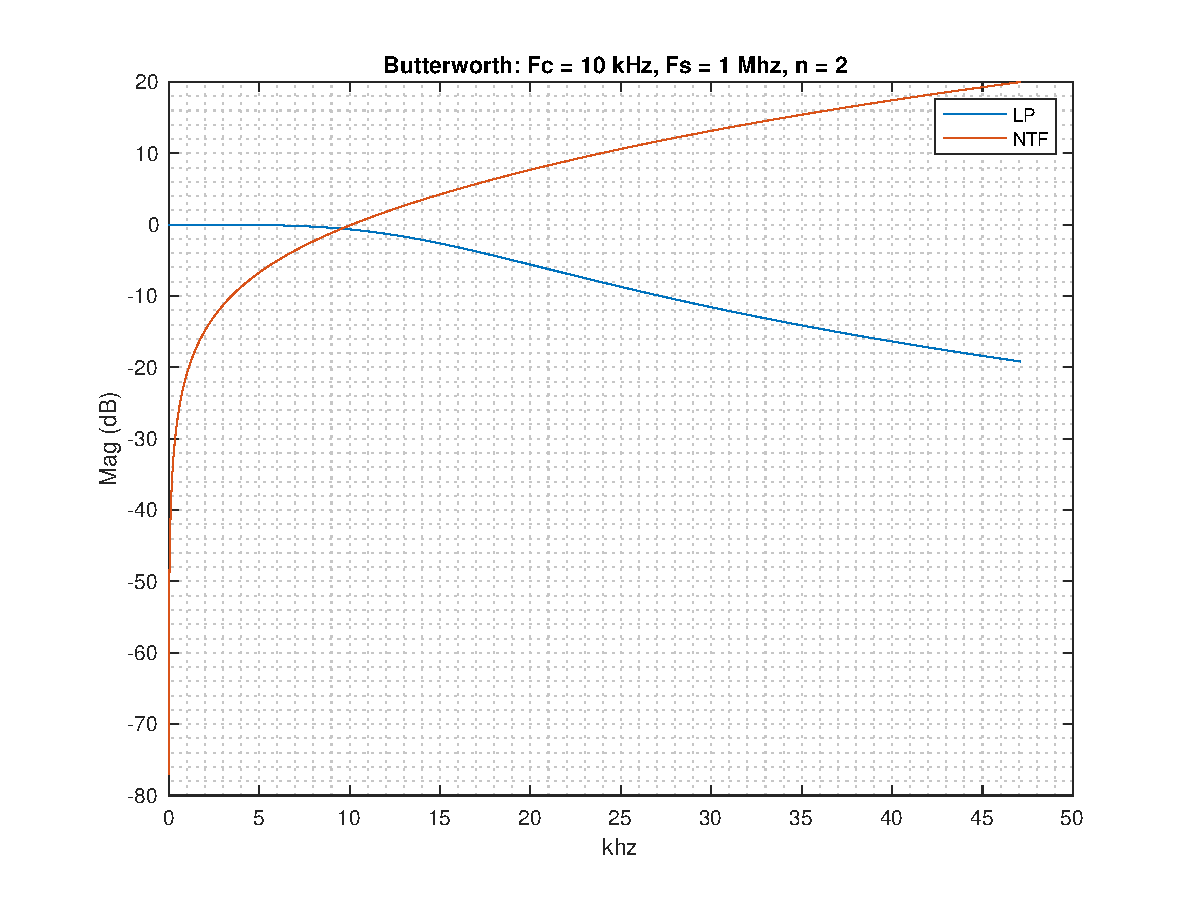
\includegraphics[scale = 0.45]{plots/but_lp_ntf_2_10.eps}
% 		\caption{Frequency response of low-pass Butterworth and  corresponding high-pass  NTF}
% 	\end{minipage}
% 	\hfil
% 	\begin{minipage}{0.45\linewidth}
% 		\centering
% 		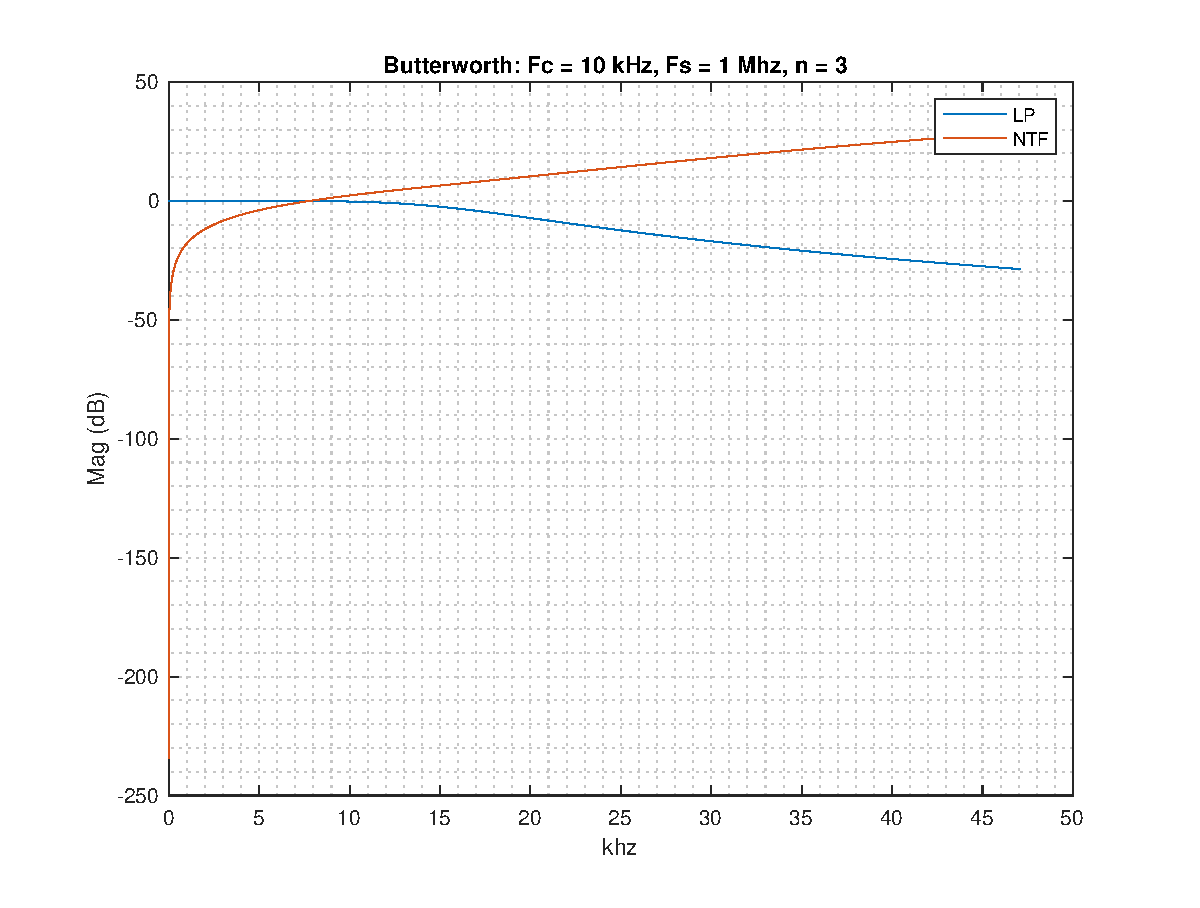
\includegraphics[scale = 0.45]{plots/but_lp_ntf_3_10.eps}
% 		\caption{Frequency response of low-pass Butterworth and  corresponding high-pass  NTF}
% 	\end{minipage}
% \end{figure}

% \begin{figure}[!h]
% 	\centering
% 	\begin{minipage}{0.45\linewidth}
% 		\centering
% 		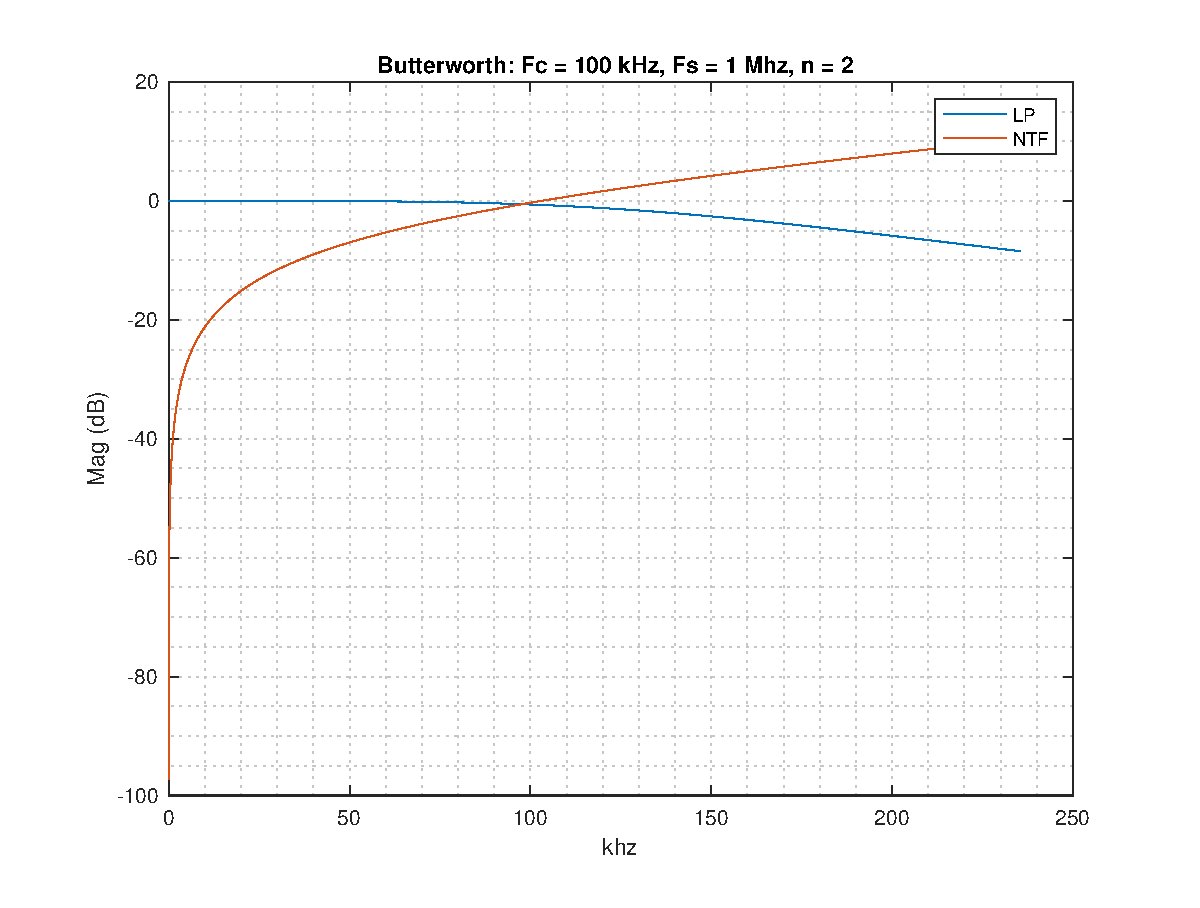
\includegraphics[scale = 0.45]{plots/but_lp_ntf_2_100_1000.eps}
% 		\caption{Frequency response of low-pass Butterworth and  corresponding high-pass  NTF}
% 	\end{minipage}
% 	\hfil
% 	\begin{minipage}{0.45\linewidth}
% 		\centering
% 		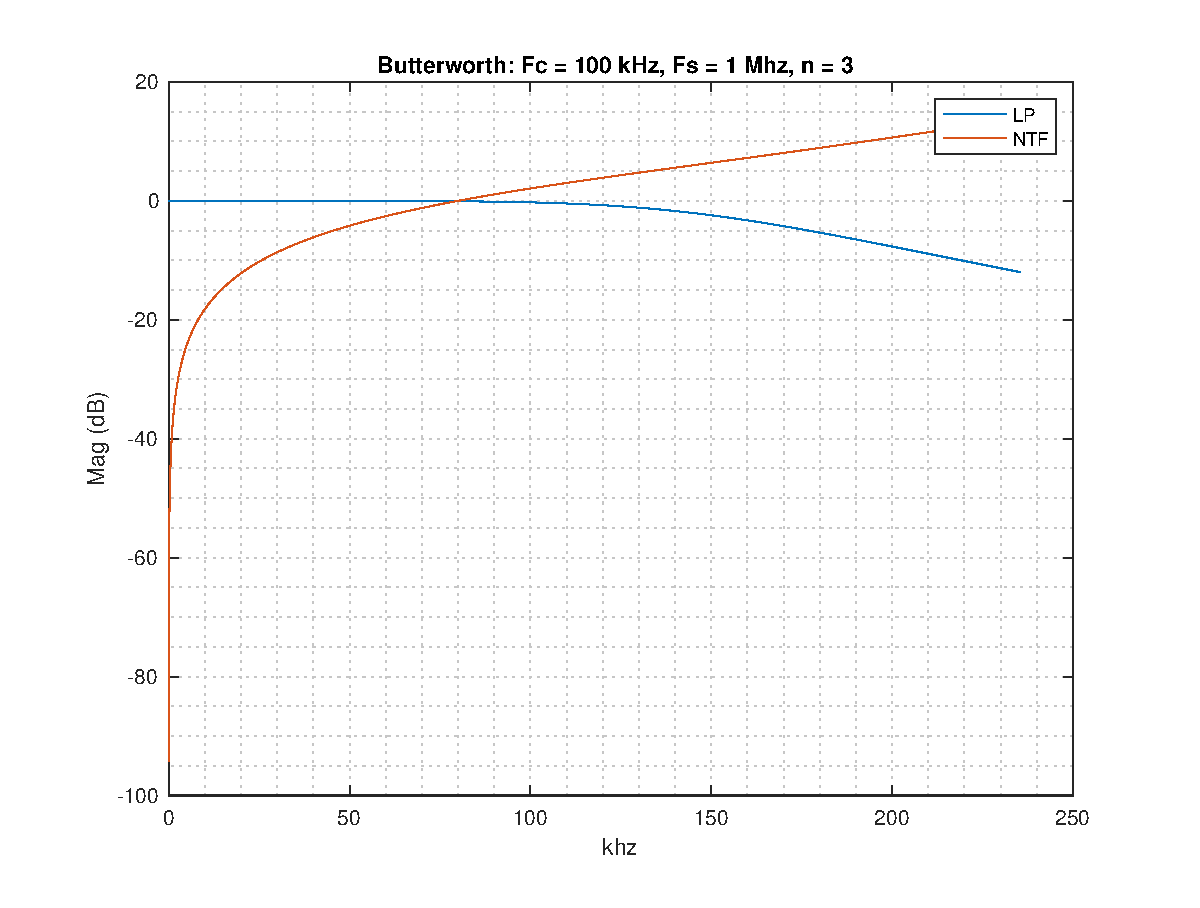
\includegraphics[scale = 0.45]{plots/but_lp_ntf_3_100_1000.eps}
% 		\caption{Frequency response of low-pass Butterworth and  corresponding high-pass  NTF}
% 	\end{minipage}
% \end{figure}


\section{Noise Transfer Function(NTF)}
The frequency response of the noise transfer functions due to butterworth filters at different cutoff frequencies are shown in the figure Fig. \ref{fig:NTFvsfreq}. In the figure, we can see that the net area under the curve remain the same.   In Fig. \ref{fig:LPFNTFvsfreq} the frequency reponse of the low pass filter is plotted along with that of the noise transefer function. This observation shows that the better performance can be achieved by increasing the cutoff frequency during MHOQ while keeping the cutoff frequency of the reconstruction as same. The simulation results in the following table confirm this observation. 

\begin{table}[!h]
	\caption{ENOB at different cutoff frequencies. Reconstruction filter: Butterworth LPF with $n =2$,  $Fc = 100 \textrm{kHz}$ and $Fs = 1\textrm{Mhz}$.}
	\centering
	\begin{tabular}{|c|c|c|c|c|c|}
	\hline
	Fc & 100 kHz & 200 kHz & 300 kHz & 400 kHz & 500 kHz \\
	\hline
	ENOB & 3.981 & 5.307 & 7.817  & 10.481 & 10.936\\
	\hline
	\end{tabular}	
	
\end{table}

\begin{figure}[!h]
	\centering
	\begin{minipage}{0.45\linewidth}
		\centering	
		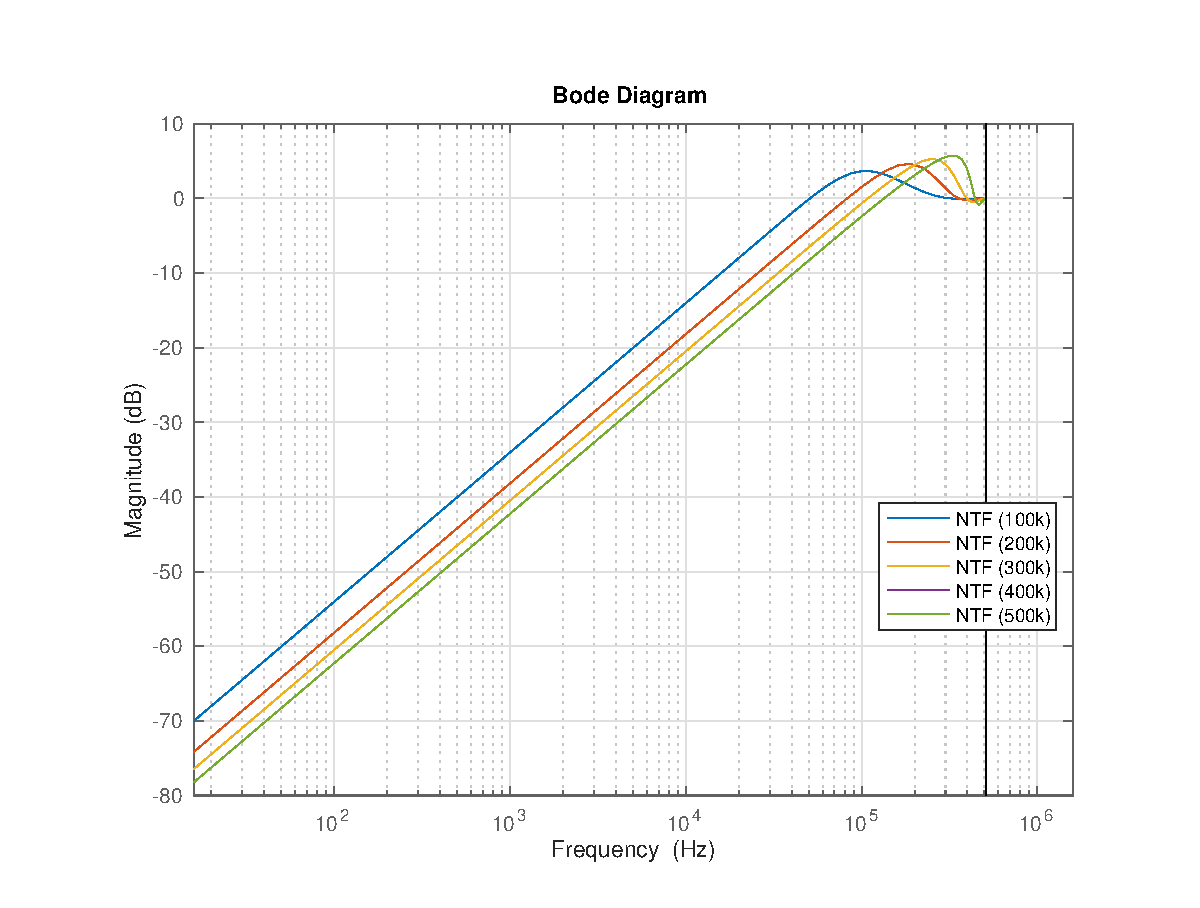
\includegraphics[scale = 0.5]{fig_stf_ntf/ntf_vs_freq.eps}
		\caption{Frequency response of NTF for different cutoff frequency}
		\label{fig:NTFvsfreq}
	\end{minipage}
	\hfil
	\begin{minipage}{0.45\linewidth}
		\centering
		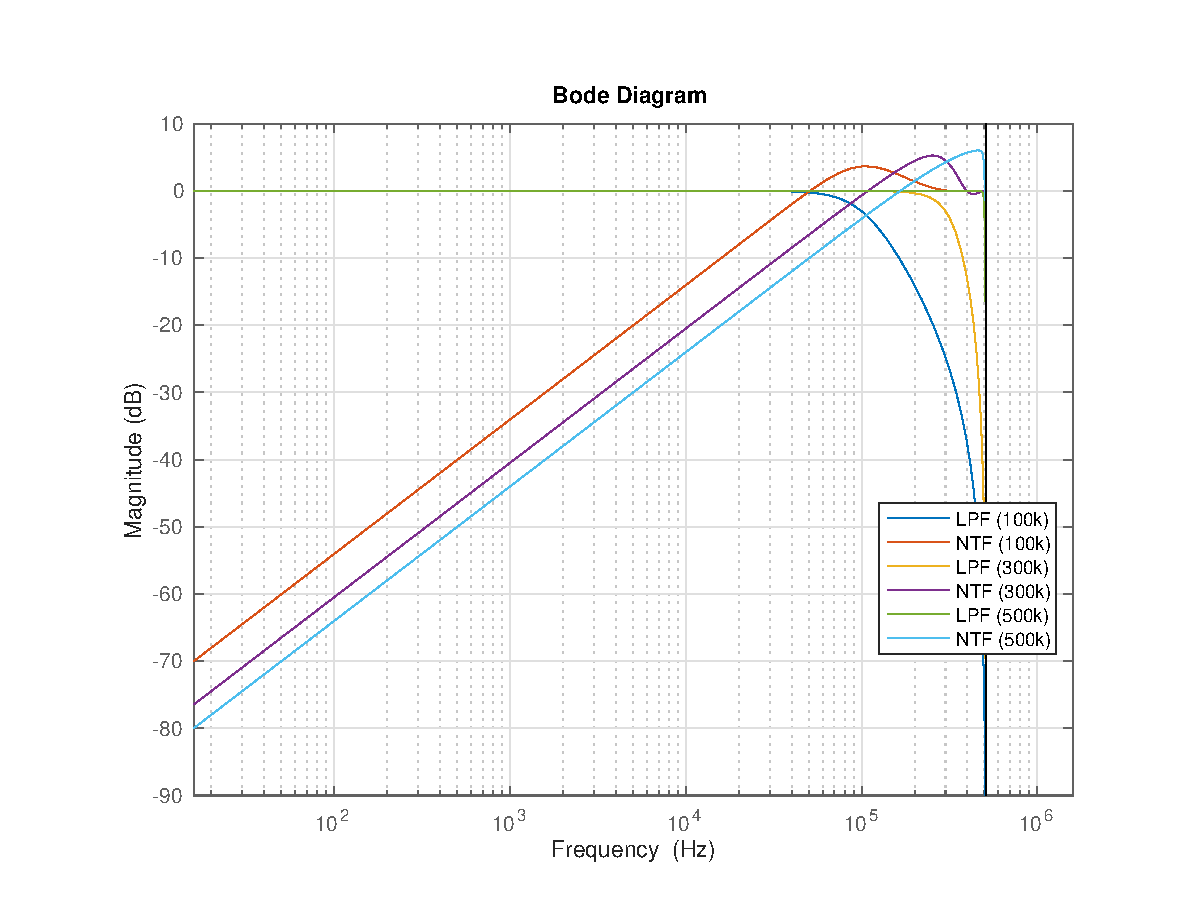
\includegraphics[scale = 0.5]{fig_stf_ntf/lpf_ntf_vs_freq.eps}
		\caption{Frequency response of LPF and NTF for different cutoff frequency}
		\label{fig:LPFNTFvsfreq}
	\end{minipage}
\end{figure}


% \begin{figure}[!h]
% 	\centering
% 	\begin{minipage}{0.45\linewidth}
% 		\centering
% 		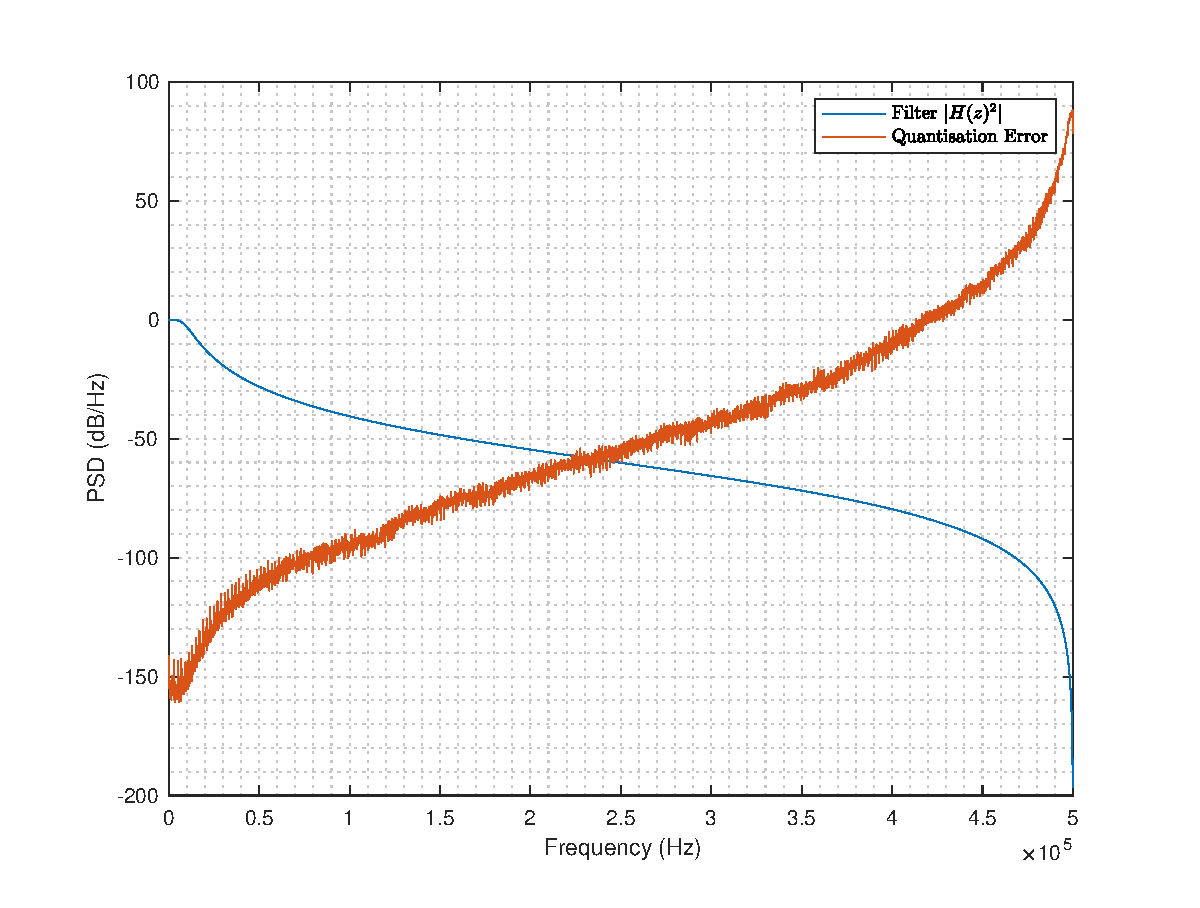
\includegraphics[scale = 0.45]{plots/quant_err_butter_2nd_10k_1mhz_inl.eps}
% 		\caption{Butterworth Frequency response and frequency spectrum of quantisation noise:  
% 				\\ \textbf{Fc} = 10 kHz, \textbf{Fs} = 1 MHz, \textbf{ENOB} = 18.47, \textbf{Uniform}}
% 	\end{minipage}
% 	\hfil
% 	\begin{minipage}{0.45\linewidth}
% 		\centering
% 		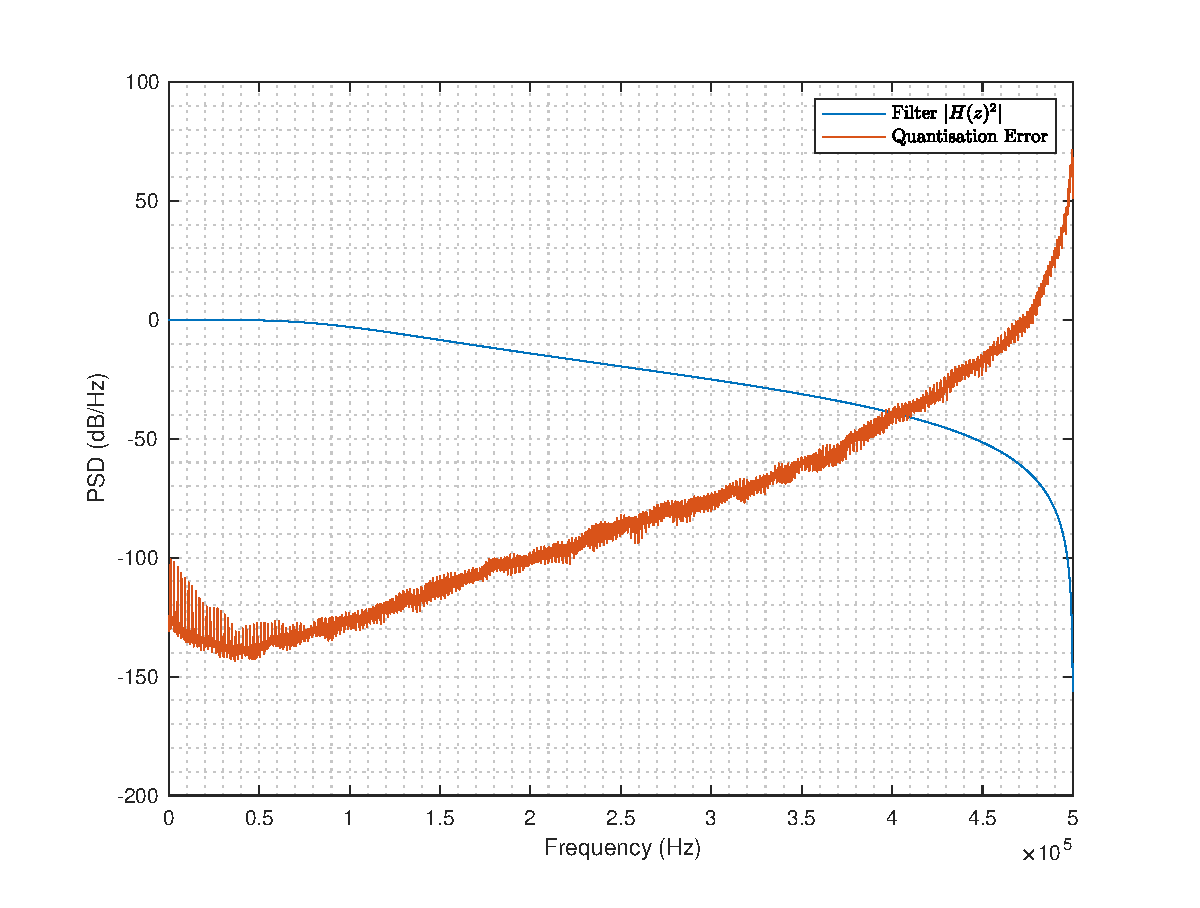
\includegraphics[scale = 0.45]{plots/quant_err_butter_2nd_100k_1mhz_ideal.eps}
% 		\textbf{\caption{Butterworth Frequency response  and frequency spectrum of quantisation noise:  
% 					\\ \textbf{Fc} = 100 kHz, \textbf{Fs} = 1 MHz, \textbf{ENOB} = 9.09, \textbf{Uniform}
% 				}}
% 	\end{minipage}
% \end{figure}

% \begin{figure}[!h]
% 	\centering
% 	\begin{minipage}{0.45\linewidth}
% 		\centering
% 		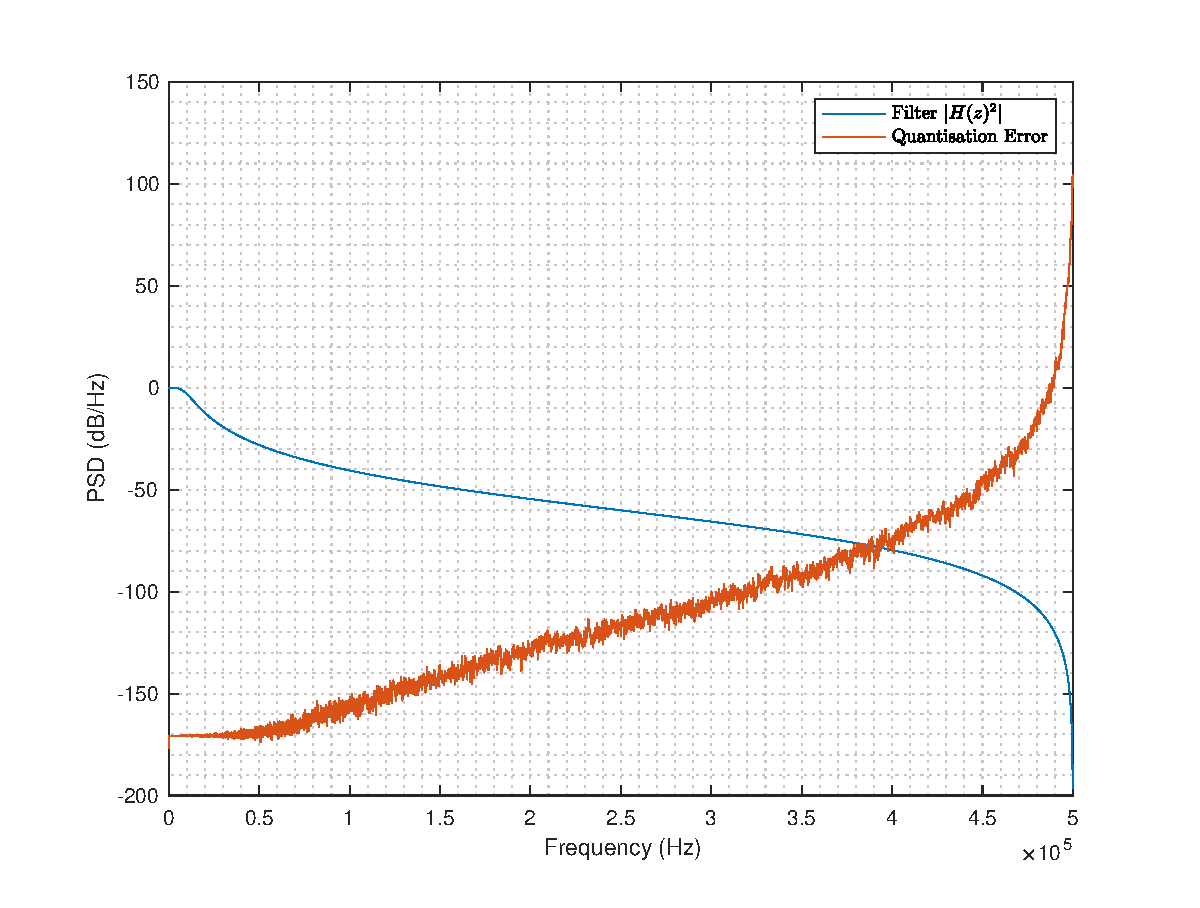
\includegraphics[scale = 0.45]{plots/filt_vs_qnoise_10k_fs10mhz_ideal.eps}
% 		\caption{Butterworth Frequency response and frequency spectrum of quantisation noise:  
% 				\\ \textbf{Fc} = 10 kHz, \textbf{Fs} = 10 MHz, \textbf{ENOB} = 26.2, \textbf{Uniform}
% }
% 	\end{minipage}
% 	\hfil
% 	\begin{minipage}{0.45\linewidth}
% 		\centering
% 		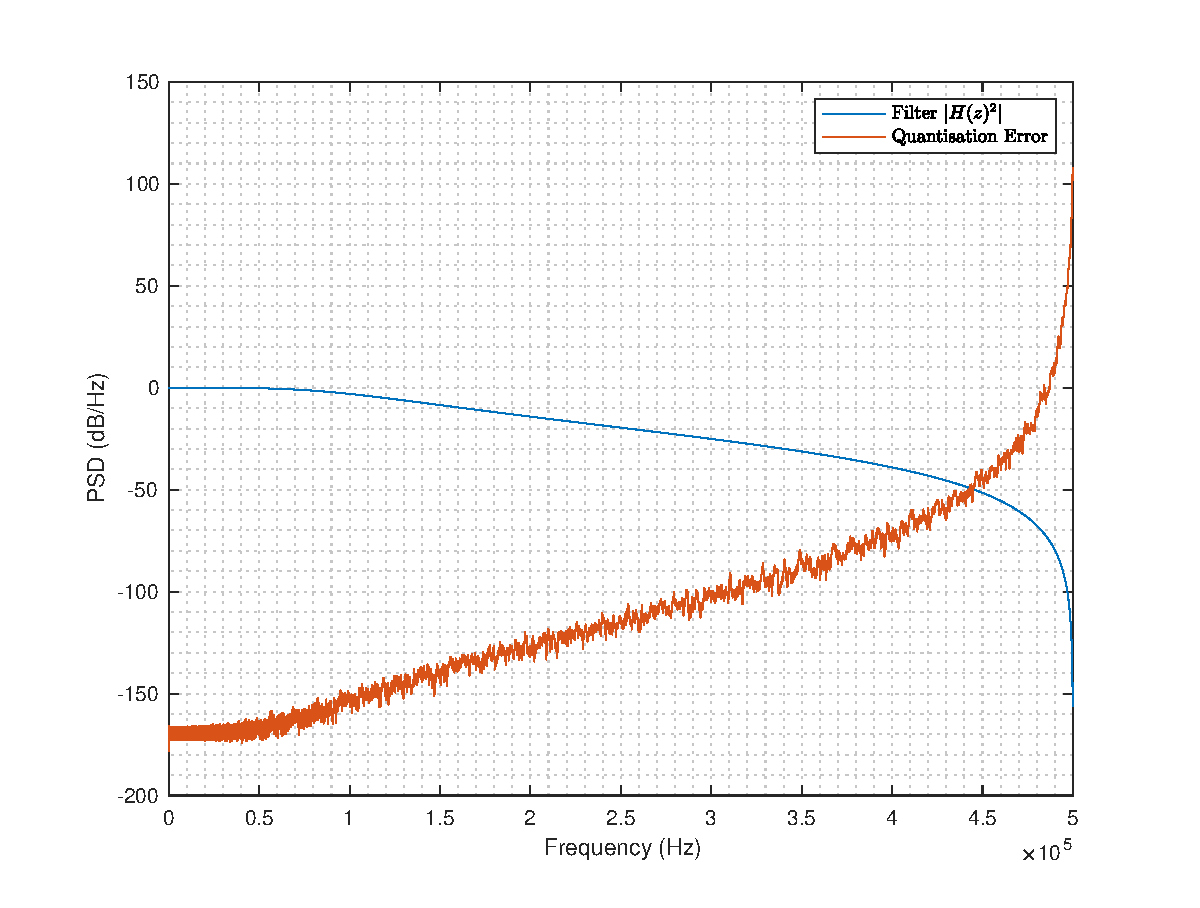
\includegraphics[scale = 0.45]{plots/filt_vs_qnoise_100k_fs10mhz_ideal.eps}
% 		\textbf{\caption{Butterworth Frequency response  and frequency spectrum of quantisation noise: 
% 					\\ \textbf{Fc} = 100 kHz, \textbf{Fs} = 10 MHz, \textbf{ENOB} = 17.31, \textbf{Unifrom}
% }}
% 	\end{minipage}
% \end{figure}
\newpage
\section{Spectrum of quantisation noise}
The sampling frequency effects the spectrum of the quantisation noise and consequently the ENOB as shown in the following figures. 

\begin{figure}[!h]
	\centering
	\begin{minipage}{0.45\linewidth}
		\centering
		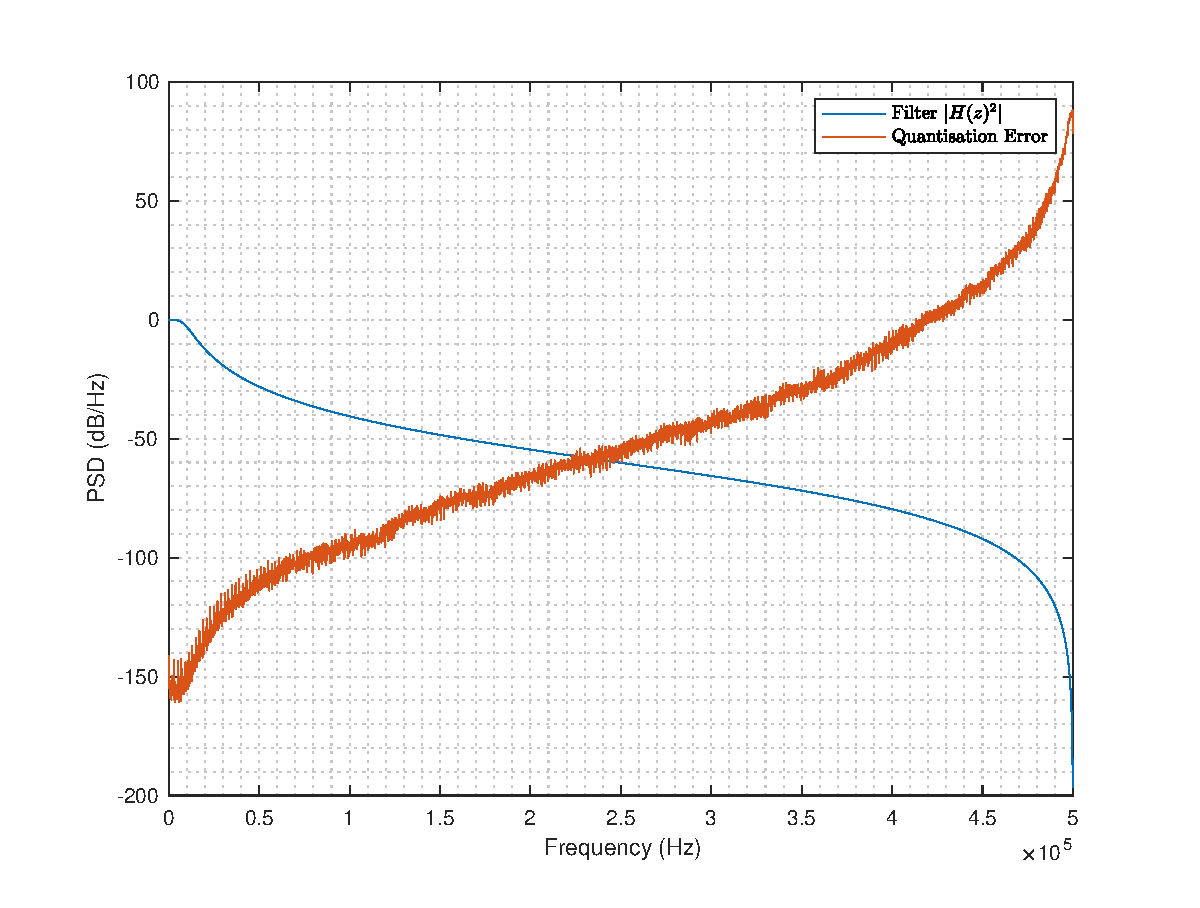
\includegraphics[scale = 0.45]{plots/quant_err_butter_2nd_10k_1mhz_inl.eps}
		\caption{Butterworth Frequency response and frequency spectrum of quantisation noise:  
			\\ \textbf{Fc} = 10 kHz, \textbf{Fs} = 1 MHz, \textbf{ENOB} = 16.58, \textbf{INL} }
	\end{minipage}
	\hfil
	\begin{minipage}{0.45\linewidth}
		\centering
		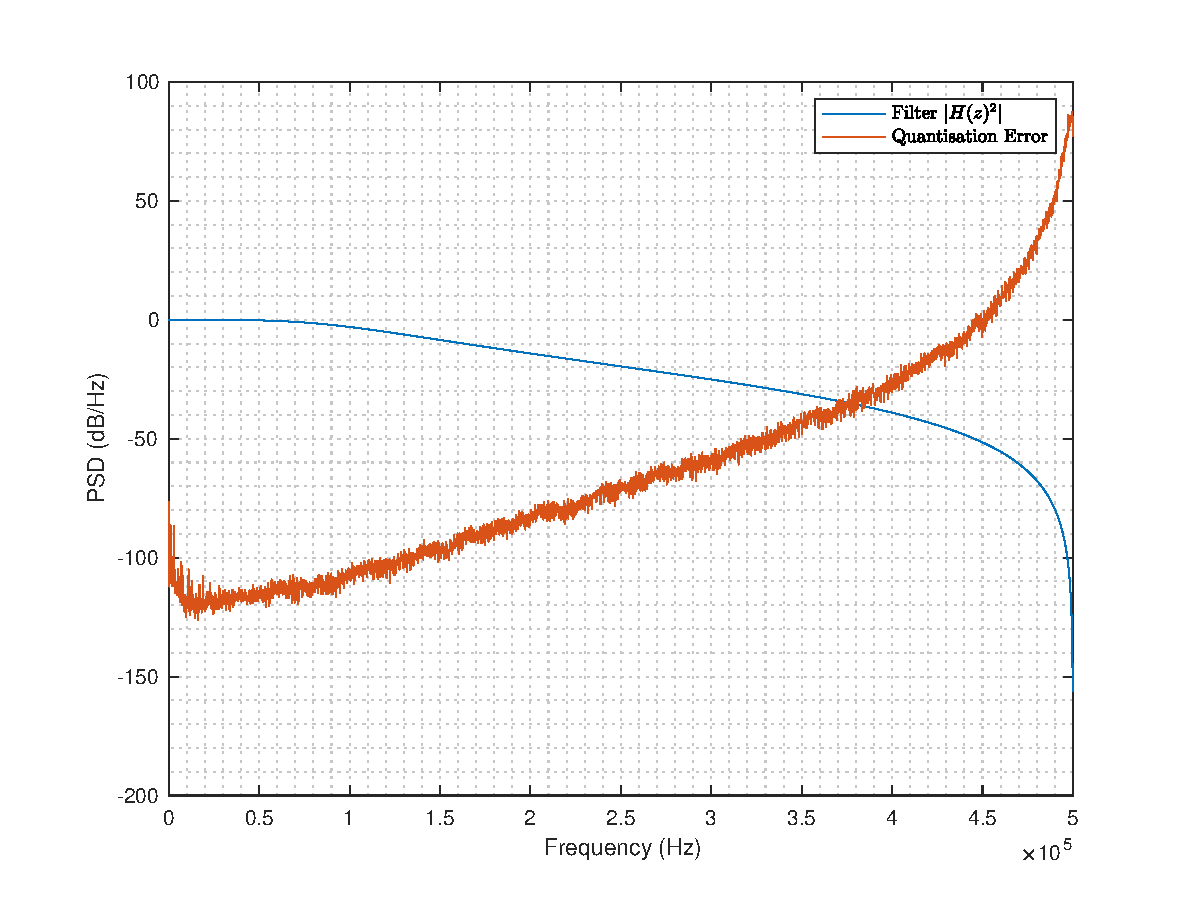
\includegraphics[scale = 0.45]{plots/quant_err_butter_2nd_100k_1mhz_inl.eps}
		\textbf{\caption{Butterworth Frequency response  and frequency spectrum of quantisation noise: 
					\\ \textbf{Fc} = 100 kHz, \textbf{Fs} = 1 MHz, \textbf{ENOB} =7.43, \textbf{INL}
 }}
	\end{minipage}
\end{figure}

\begin{figure}[!h]
	\centering
	\begin{minipage}{0.45\linewidth}
		\centering
		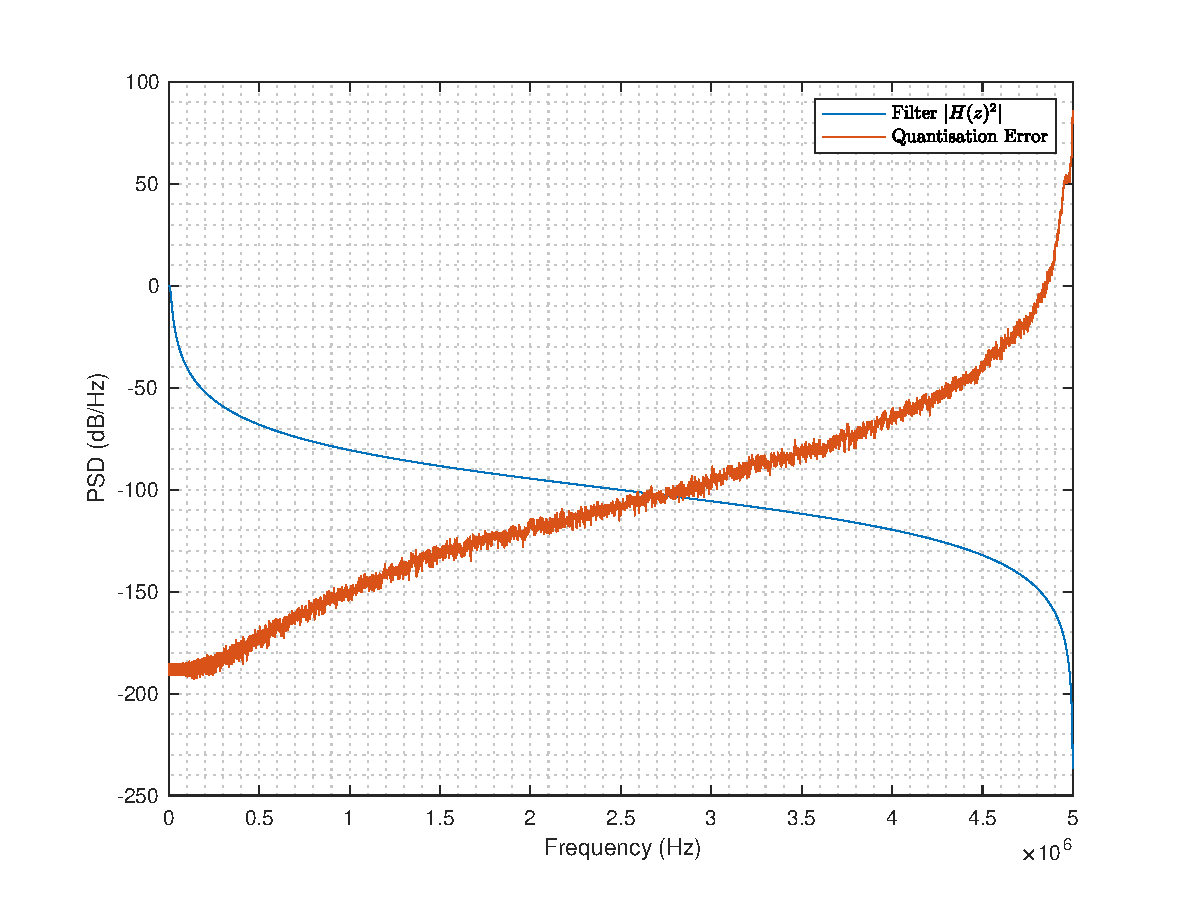
\includegraphics[scale = 0.45]{plots/quant_err_butter_2nd_10k_10mhz_inl.eps}
		\caption{Butterworth Frequency response and frequency spectrum of quantisation noise: 
		\\ \textbf{Fc} = 10 kHz, \textbf{Fs} = 10 MHz, \textbf{ENOB} = 25.12, \textbf{INL}}
	\end{minipage}
	\hfil
	\begin{minipage}{0.45\linewidth}
		\centering
		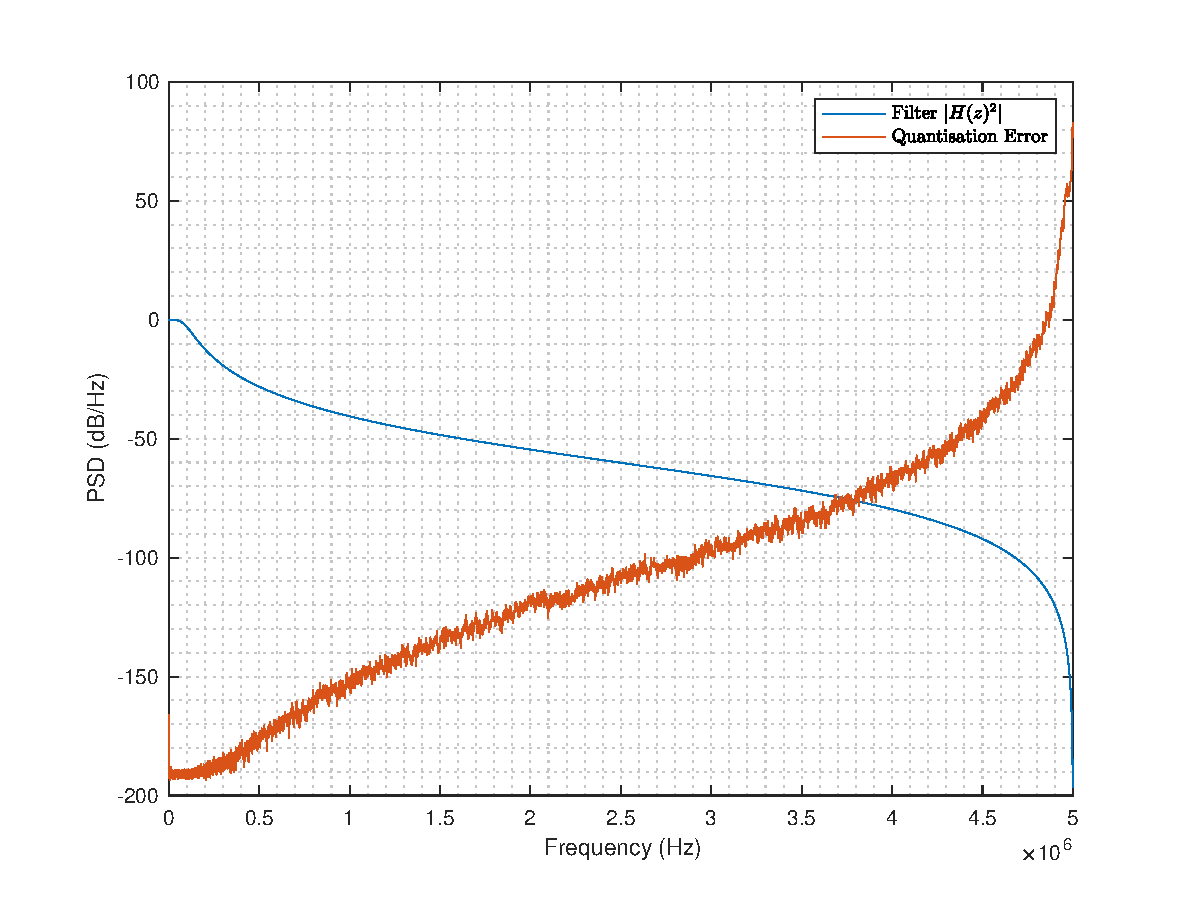
\includegraphics[scale = 0.45]{plots/quant_err_butter_2nd_100k_10mhz_inl.eps}
		\textbf{\caption{Butterworth Frequency response  and frequency spectrum of quantisation noise:  
			\\ \textbf{Fc} = 100 kHz, \textbf{Fs} = 10 MHz, \textbf{ENOB} = 17.03, \textbf{INL}	
 }}
	\end{minipage}
\end{figure}

\newpage
\section{Synthesis of optimal noise-shaping filter}

\begin{figure}[!h]
	\centering
	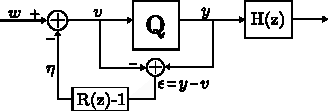
\includegraphics[scale = 2]{figures/nsq_error_feedback.pdf}
	\caption{Noise shaping quantiser and a filter $H(z)$.}
	\label{fig:nsq_efs}
\end{figure}
In noise shaping quantiser with error-feedback structure as shown in the Figure \ref{fig:nsq_efs}, the input to the quantiser is  $v = w + \eta = w + (R(z)-1)\epsilon$
and  feedback error $\epsilon$ is 
\begin{equation}
	\epsilon = y - v = y - w - (R(z)-1)\epsilon.
\end{equation}

Then quantisaion noise defined as $q := y - w$ can be expressed as 
\begin{equation}
	 q = y - w = R(z) \epsilon.
\end{equation}
Then the effect of the quantisation error on the system $H(z)$ can be expressed as 
\begin{equation}	
	 e = H(z) R(z) \epsilon.
	 \label{eq:err_plant}
\end{equation}
and it shows that we can reduce the error in the plant output by properly designing the noise shaping filter $R(z)$ with the knowledge of the plant $H(z)$. 

The objective is to design stable noise-shaping filter such that it minimises the effect of the quantisation noise in the plant output. A constraint on the error feedback signal should be imposed to prevent the quantiser from overloading and achieve a stable noise-shaping quantiser as $$ \eta = (R(z) - 1) \epsilon.$$

\begin{itemize}
	\item \textbf{Design Problem:} For a fixed pair (p,q) \cite{Shuichi2017}, 
	\begin{equation}
		\begin{aligned}
			&\min_{R(z) \in \mathbb{RH}_{\infty}} \| e \|_{p}  \\
			\textrm{subject  to.}& \\
			& R(\infty)	 = 1, \\
			& \|\eta\|_{q} < \gamma_{\eta}
		\end{aligned}	
	\end{equation}	
	where $\mathbb{RH}_{\infty} = \mathbb{R} \cap \mathbb{H}_{\infty}$ is the set of proper stable rational transfer functions.
\end{itemize}

\subsection{Solution 1: Optimal noise shaping filter without constraint}
The optimal noise shaping filter without constraint on the error feedback signal $\eta$ is the scaled inverse of the system $H(z)$.   If the quantisation error is assumed to be an i.i.d random variable with zero mean, then the variance of the error $e$ at time $k$  can be expressed as 
\begin{equation}
	E\{|e_{k}|^2\} = \|H(z) R(z) \|_{2}^{2} \sigma_{\epsilon}^{2}
\end{equation}
where $E\{.\}$ is the expectation operator and $\sigma_{\epsilon}$ is variance of the $\epsilon$ and $\|H(z) R(z) \|_{2}^{2}$  is the $\mathbb{H}_{2}$-norm.

It is shown in \cite{oppenheim99}, any casual and stable rational sytem function $H(z)$ can always be stated as the product of the minimum phase system $H_{min}(z)$ and all pass system $H_{ap}(z)$. Then it is shown that the optimal noise shaping filter is given by the scaled inverse of the plant, as follows, 
\begin{equation}
	R(z) = h_{D} H_{min}^{-1}(z)
\end{equation}
where $h_{D}$ is the first non-zero entry of the impulse response of the plant $H_{z}$.

\subsection{Solution 2: Optimal noise shaping filter with constraint}
The optimization problem is setup as the minimization of the upper bound of the $\|e\|_{p}$ and $\|\eta_{q}$ as follows:
\begin{align}
	\min_{R(z) \in \mathbb{RH}_{\infty}}\gamma_{e} \\
	\intertext{subject to $R(\infty) = 1$ and}
	\|H(z)R(z)\|_{ind.p} < \gamma_{e} \\
	\|R(z) - 1\|_{ind.q}< \gamma_{\eta}
\end{align}
where $\|.\|_{ind.r}$ is the induced norm and $\gamma_{e}$ and $\gamma_{\eta}$ are the upper bound of $\|H(z)R(z)\|_{ind.p}$ and $\|R(z) - 1\|_{ind.q}$ , respectively.

\subsubsection*{State space representation}


\subsubsection{System}
Denoting the state-space representation of the $H(z)$ and $R(z)$ as $(A_{h}, B_{h}, C_{h}, D_{h})$ and $(A_{r}, B_{r}, C_{r}, 1)$ respectively, the state space realization of $H(z)R(z)$ is 
\begin{align}
	x_{k+1} &= Ax_{k} + B \epsilon_{k} \\
	e_{k} &= Cx_{k} + D\epsilon_{k}
\end{align}
where 
\begin{align}
	A = \begin{bmatrix}
		A_{h} & B_{h}C_{r}\\
		\mathbf{0} & A_{r}
	\end{bmatrix}
	\qquad
	B = \begin{bmatrix}
		B_{h} \\
		B_{r}
	\end{bmatrix}
	\qquad
	C = \begin{bmatrix}
		C_{h} & D_{h} C_{r}
	\end{bmatrix}
	\qquad
	D = D_{h}.
\end{align}
Similary, the variance of the error $e$ under the white noise assumption at time $k$ in state-space form is given by $\mathbb{H}_{2}$-norm  as
\begin{equation}
	\|H(z)R(z)\|_{2}^{2} = \sum_{k = 0}^{\infty} \|C A^{k}B\|_{2}^{2} + DD^{\top}.
\end{equation}
Moreover, if $A$ is Schur matrix, then there exists a positive semi-definite solution $P$ of the discrete Lyapunov equation defined as 
\begin{equation}
	P = A^{\top} P A + B B^{\top}
\end{equation}
and the squared $\mathbb{H}_{2}$ norm is given by
\begin{equation}
		\|H(z)R(z)\|_{2}^{2} = C P C^{\top} + D D^{\top}.
\end{equation}
\subsubsection{Constraint 1}
Then $\|H(z) R(z)\|_{2} < \gamma_{e}$ if and only if there exist a positive definite matrix $P$ such that 
\begin{align}
	 \mathbf{(BMI)} \qquad &\begin{bmatrix}
		P & PA & PB \\
		A^{\top} & P & \mathbf{0} \\
		B^{\top} & \mathbf{0} & 1
	\end{bmatrix} \succ 0 \\
	\mathbf{(LMI)} \qquad &\begin{bmatrix}
		\mu_{e} & C & D \\
		C^{\top} & P & \mathbf{0} \\
		D^{\top} & \mathbf{0} & 1
	\end{bmatrix} \succ 0 \\
&\mu_{e} = \gamma_{e}^{2}.
\end{align}

\subsubsection{Constraint 2}
 The variance of the noise shaping filter is given by
 \begin{equation}
	E\{|\eta_{k}|^{2}\} = \|R(z)-1 \|_{2}^{2} = \sum_{k = 1}^{\infty} \|\tilde{C} A^{k} B\|_{2}^{2},
 \end{equation}
 where  $\tilde{C} = \begin{bmatrix}
	\mathbf{0} & C_r
 \end{bmatrix}$. Then $\|R(z)-1 \|_{2}^{2} < \gamma_{\eta}$ if and only if there exist a  positive definite matrix $P$ that satisfies
\begin{align}
	 \mathbf{(BMI)} \qquad &\begin{bmatrix}
		P & PA & PB \\
		A^{\top} & P & \mathbf{0} \\
		B^{\top} & \mathbf{0} & 1
	\end{bmatrix} \succ 0 \\
	\mathbf{(LMI)} \qquad &\begin{bmatrix}
		\mu_{\eta} & \tilde{C} \\
		\tilde{C}^{\top} & P 
	\end{bmatrix} \succ 0 \\
&\mu_{\eta} = \gamma_{\eta}^{2}.
\end{align}

\subsubsection{Optimization problem: State Space formulation}
Thus the optimization problem can be written as follows, 
\begin{align}	
	\min_{R(z) \in \mathbb{RH}_{\infty}}\gamma_{e} \\
	\intertext{subject to $R(\infty) = 1$ and}
	 &\begin{bmatrix}
		P & PA & PB \\
		A^{\top} & P & \mathbf{0} \\
		B^{\top} & \mathbf{0} & 1
	\end{bmatrix} \succ 0  \label{eq:bmi1}\\
	\qquad &\begin{bmatrix}
		\mu_{e} & C & D \\
		C^{\top} & P & \mathbf{0} \\
		D^{\top} & \mathbf{0} & 1
	\end{bmatrix} \succ 0 \label{eq:lmi1}\\	
	&\begin{bmatrix}
		\mu_{\eta} & \tilde{C} \\
		\tilde{C}^{\top} & P 
	\end{bmatrix} \succ 0 \label{eq:lmi2}\\
&\mu_{e} = \gamma_{e}^{2} , \mu_{\eta} = \gamma_{\eta}^{2}. \label{eq:lmi3}
\end{align}

\section{LMI Synthesis: Convert BMIs to convex LMIs}
BMIs are not convex and NP hard to solve, but they can be converted to convex LMIs  and can be solved numerically whereas the LMIs are convex. The non-convex BMIs can be converted to convex LMIs using change of variables \cite{Izumi1998}. 
\subsection*{Change of Variables:}
Let the order of $H(z)$ is $n$ and the set of $n \times n$ positive define matrices is denoted as $\textrm{PD}(n)$. Denote by $\mathcal{P}$ the set of variables $\mathbf{p} = \{P_{f}, P_{g}, W_{f}, W_{g}, W_{h}, L\}$ where $P_{f} \in \textrm{PD}(n)$,  $P_{g} \in \textrm{PD}(n)$, $W_{f} \in \mathbb{R}^{1 \times n}$,  $W_{g} \in \mathbb{R}^{n \times 1}$, $W_{h} \in \mathbb{R}$ and $L \in \mathbb{R}^{n \times n}$. Then define the following matrix values function on $\mathcal{P}$:
\begin{equation}
	\begin{aligned}
		M_{A}&:= \begin{bmatrix}
			A_{h} P_{f} + B_{h} W_{f} & A_{h} \\
			L & P_{g} A_{h}
		\end{bmatrix} \\
		M_{B} &:= \begin{bmatrix}
			B_{h} \\ W_{g}
		\end{bmatrix} \\
		M_{C} &:= \begin{bmatrix}
			C_{h}P_{f} + D_{h}W_{f} & C_{h}
		\end{bmatrix} \\
		M_{P} &:= \begin{bmatrix}
			P_{f} & I_{n} \\
			I_{n} & P_{g}
		\end{bmatrix}.
	\end{aligned}	
\end{equation}
Next, define 
\begin{align}
	{P}^{-1} &:= \begin{bmatrix}
		P_{f} & S_{f} \\
		S_{f} & S_{f}
	\end{bmatrix} ,
	\qquad
	U := \begin{bmatrix}
		P_f & I_{n} \\
		S_{f} & \mathbf{0}
	\end{bmatrix} \qquad \textrm{and} \\
	S_{f} &:= P_{f} - P_{g}^{-1} ( \succ 0)
\end{align}
then we have, 
\begin{equation}
	M_{P} = U^{\top} {P} U.
\end{equation}
If the matrices $(A_{r}, B_{r}, C_{r})$ are given by 
\begin{equation}
	\begin{aligned}
		A_{r} &:= \begin{bmatrix}
			B_{h} W_{f} - P_{g}^{-1}(L - P_g A_h P_f)
		\end{bmatrix} S_{f}^{-1} \\
		B_{r} &:= \begin{bmatrix}
			B_{h} - P_g^{-1}W_{g}
		\end{bmatrix}\\
		C_{r} &:= W_{f}S_{f}^{-1}
	\end{aligned}
\end{equation}
then $(A, B, C)$ satisfy, 
\begin{align}
	M_{A} &= U^{\top}P A U \\
	M_{B} &= U^{\top}P B\\
	M_{C} &=  C U \\
	M_{p} &= U^{\top}PU.
\end{align}
Multiplying with the transformation $\phi = \textrm{diag}(U, U, 1)$ form the RHS and $\phi^{\top}$  from the LHS the BMI condition \ref{eq:bmi1} takes the following form:
\begin{equation}
	\begin{bmatrix}
		M_{P} & M_{A} & M_{B}\\
		M_{A}^{\top} & M_{P} & \mathbf{0} \\
		M_{B}^{\top} & \mathbf{0} & \mathbf{I}
	\end{bmatrix} \succ 0.
	\label{eq:bmi21}
\end{equation}
Similarly, using the transformation $\textrm{diag}(1, U, 1)$, the LMI condition \ref{eq:lmi1} is 
\begin{equation}
	\begin{bmatrix}	
	\mu_{e} & M_{C} & D^{\top} \\
	M_{C}^{\top} & M_{P} & \mathbf{0} \\
	D & \mathbf{0} & \mathbf{I}
	\end{bmatrix} \succ 0
	\label{eq:lmi22}
\end{equation}
and finally the constraint \ref{eq:lmi2} using the transformation is 
\begin{equation}
	\begin{bmatrix}
		\gamma_{\eta}^{2} & M_{\tilde{C}} \\
		M_{\tilde{C}}^{\top} & M_{P}
	\end{bmatrix} \succ 0 \label{eq:lmi23}
\end{equation}
with $M_{\tilde{C}} := \tilde{C}U$. The LMI conditions  \ref{eq:bmi21}, \ref{eq:lmi22} and \ref{eq:lmi23} are convex and the minimization of $\gamma_{e}$ with these constraints is a convex optimization problem.

\subsection{Optimization Problem:}
With the change of the variable the BMI is converted to the LMI and the since all the LMIs are convex the optimization problem is a convex optimization problem. Also, since the objective is linear and the constraints are LMIs and linearity constraints, the optimization problem is SemiDefinite Program (SDP). Such SDP can be solved numerically using CVX. The optimization problem takes the following form, 
\begin{align}
	&\min \mu_{e} = \gamma_{e}^{2} \\
	\intertext{subject to,} 	
	&\begin{bmatrix}
		M_{P} & M_{A} & M_{B}\\
		M_{A}^{\top} & M_{P} & \mathbf{0} \\
		M_{B}^{\top} & \mathbf{0} & \mathbf{I}
	\end{bmatrix} \succ 0 \label{eq:sdpcons1} \\
	&\begin{bmatrix}	
	\mu_{e} & M_{C} & D^{\top} \\
	M_{C}^{\top} & M_{P} & \mathbf{0} \\
	D & \mathbf{0} & \mathbf{I}
	\end{bmatrix} \succ 0 . \label{eq:sdpcons2} \\
	&\begin{bmatrix}
		\mu_{\eta} & M_{\tilde{C}} \\
		M_{\tilde{C}}^{\top} & M_{P}
	\end{bmatrix} \succ 0 \label{eq:sdpcons3}
\end{align}
where $\mu_{e}$ is the variance of the output error  and $\mu_{\eta} $ the variance of the feedback error. 


\section{Simulatino: Butterworth LPF}
Let us consider a second order butterworth low pass filter with $F_c = 100 \mathit{kHz}$  and $F_s = 1 \mathit{Mhz}$. Also, denote the low pass filter as $H(z)$ then let $F_{opt}(z)$ as the optimal noise transfer function and $F_{mpc}(z)$ as the noise transfer function due to MPC setting i.e. $F_{mpc} = (H(z)-1)/H(z)$ and  the numerator and denominator of noise transfer function $R(z)$ as $b_{r}$ and $a_{r}$, respectively, i.e., 
% \begin{align}
	$R(z) = b_{r}/a_{r}.$
% \end{align}
Then the corresponding noise shaping filter (NSF) as shown in the Figure~\ref{fig:nsq_efs}  is 
\begin{align}	
F(z)  = 1- R(z)= \frac{a_{r}- b_{r}}{a_{r}}.
\end{align}
Following the analogy of MPC formualation the obtained low pass filter due the high- noise shaping filter is 
\begin{equation}
	H_{mpc}(z) = \frac{1}{1-F(z)} =  \frac{a_{r}}{b_{r}}.
\end{equation}  
% \begin{figure}[!h]
% 	\centering
% 	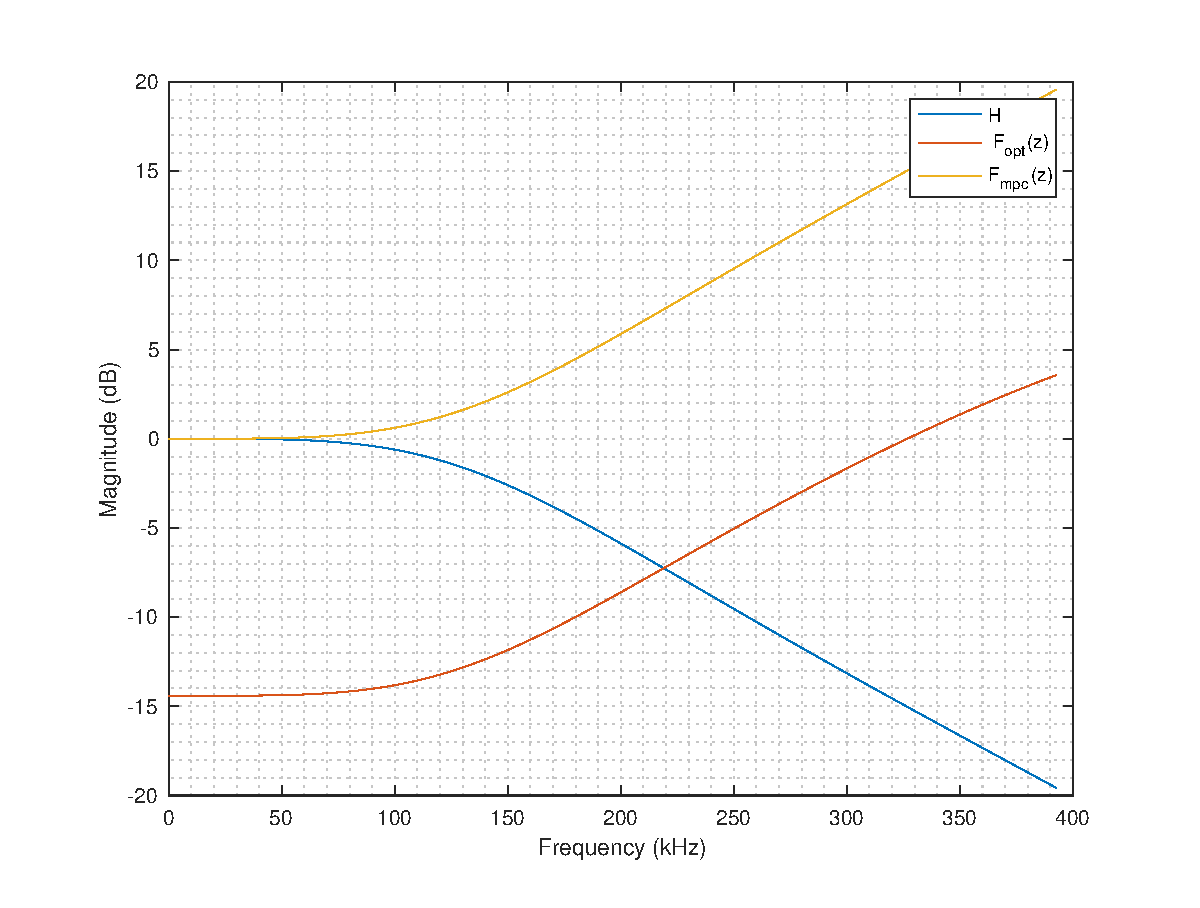
\includegraphics[scale = 1]{mat_plots/butter_2_100khz_1Mhz.eps}	
% 	\caption{Frequency response: Butterworth filter with $n = 3$ and $F_{c} = 100\mathit{kHz}$}
% \end{figure}


\begin{figure}[!h]
	\centering
	\begin{minipage}{0.45\linewidth}
		\centering
		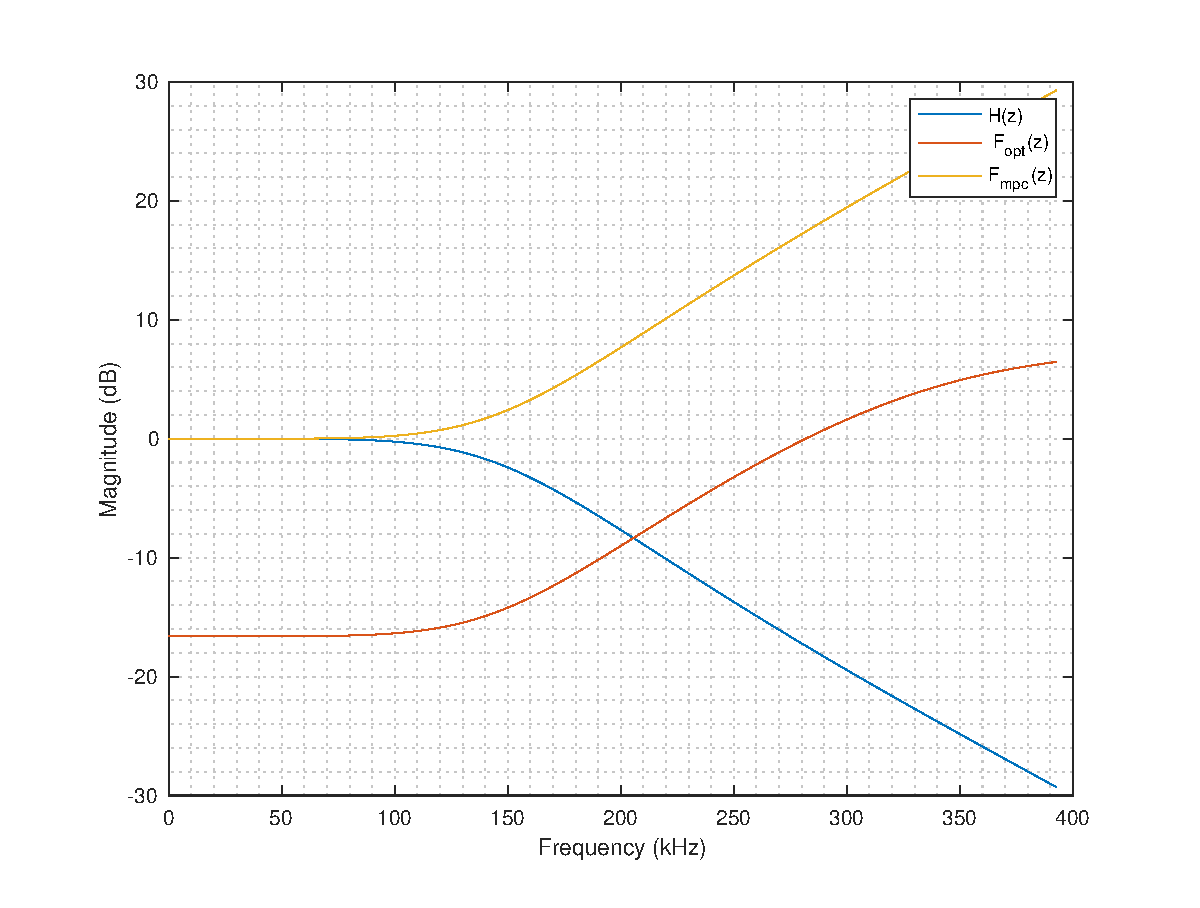
\includegraphics[scale = 0.45]{mat_plots/butter_3_100khz_1Mhz_1.eps}
		\caption{Frequency response: Butterworth filter with $n = 3$ and $F_{c} = 100\mathit{kHz}$ and corresponding optimal noise shaping filter and low pass filter}
	\end{minipage}
	\hfil
	\begin{minipage}{0.45\linewidth}
		\centering
		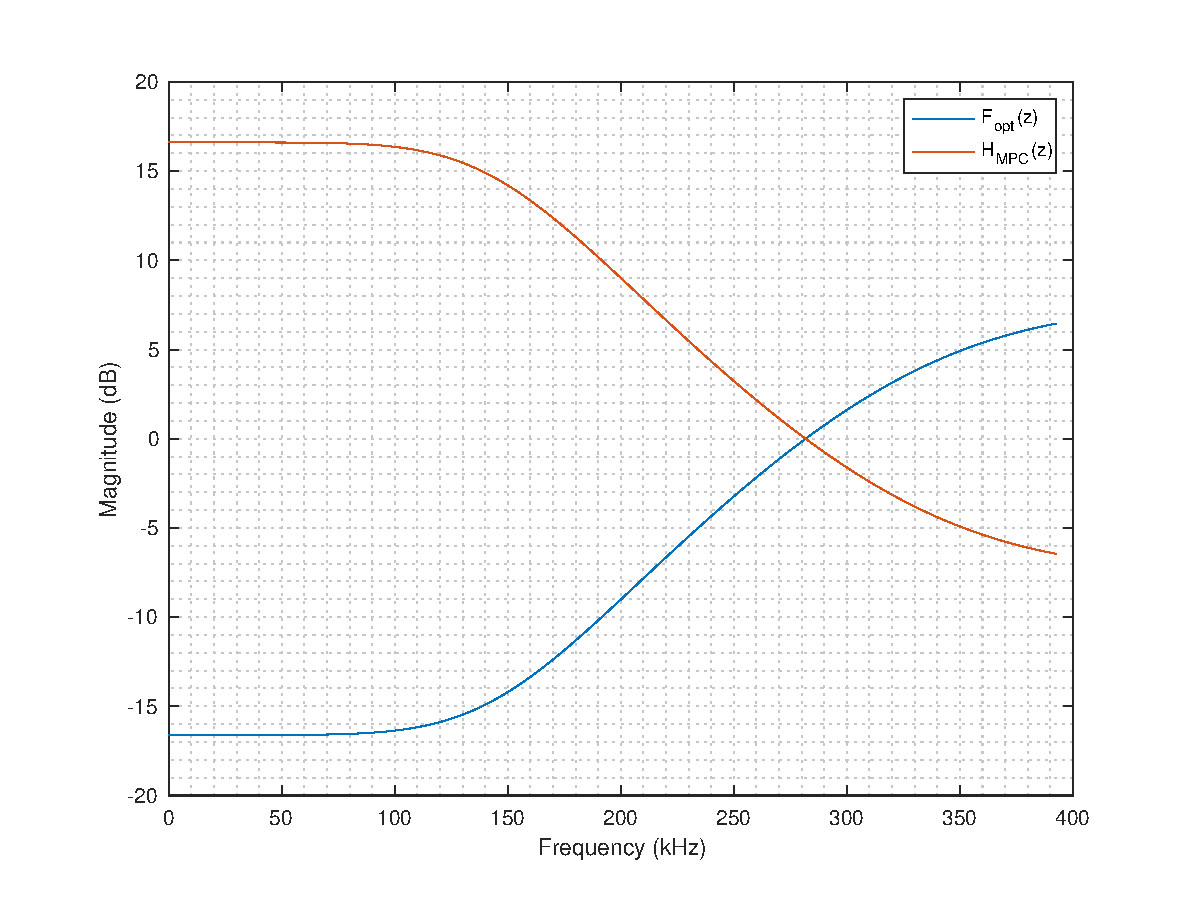
\includegraphics[scale = 0.45]{mat_plots/butter_3_100khz_1Mhz_2.eps}
		\caption{Frequency response: Optimal noise shaping filter and corresponding low pass filter}
	\end{minipage}
\end{figure}

\newpage
%\section{References}
%\label{sec:org89add8d}
\bibliographystyle{unsrt}
\bibliography{references_new} 
\end{document}